% ******************************************************** %
%              TEMPLATE DE INFORME ORGA2 v0.1              %
% ******************************************************** %
% ******************************************************** %
%                                                          %
% ALGUNOS PAQUETES REQUERIDOS (EN UBUNTU):                 %
% ========================================
%                                                          %
% texlive-latex-base                                       %
% texlive-latex-recommended                                %
% texlive-fonts-recommended                                %
% texlive-latex-extra?                                     %
% texlive-lang-spanish (en ubuntu 13.10)                   %
% ******************************************************** %


\documentclass[a4paper]{article}
\usepackage[spanish]{babel}
\usepackage[utf8]{inputenc}
\usepackage{charter}   % tipografia
\usepackage{graphicx}
%\usepackage{makeidx}
\usepackage{paralist} %itemize inline
\usepackage{subcaption}


%\usepackage{float}
%\usepackage{amsmath, amsthm, amssymb}
%\usepackage{amsfonts}
%\usepackage{sectsty}
%\usepackage{charter}
%\usepackage{wrapfig}
%\usepackage{listings}
%\lstset{language=C}

% \setcounter{secnumdepth}{2}
\usepackage{underscore}
\usepackage{caratula}
\usepackage{url}
\usepackage{ragged2e}
\usepackage{hyperref}
\usepackage{pdfpages}
\hypersetup{
	colorlinks=true,
	linkcolor=black,
	filecolor=magenta,      
	urlcolor=cyan,
}

% ********************************************************* %
% ~~~~~~~~              Code snippets             ~~~~~~~~~ %
% ********************************************************* %

\usepackage{color} % para snipets de codigo coloreados
\usepackage{fancybox}  % para el sbox de los snipets de codigo

\definecolor{litegrey}{gray}{0.94}

\newenvironment{codesnippet}{%
	\begin{Sbox}\begin{minipage}{\textwidth}\sffamily\small}%
	{\end{minipage}\end{Sbox}%
		\begin{center}%
		\vspace{-0.4cm}\colorbox{litegrey}{\TheSbox}\end{center}\vspace{0.3cm}}



% ********************************************************* %
% ~~~~~~~~         Formato de las páginas         ~~~~~~~~~ %
% ********************************************************* %

\usepackage{fancyhdr}
\pagestyle{fancy}

%\renewcommand{\chaptermark}[1]{\markboth{#1}{}}
\renewcommand{\sectionmark}[1]{\markright{\thesection\ - #1}}

\fancyhf{}

\fancyhead[LO]{Sección \rightmark} % \thesection\ 
\fancyfoot[LO]{\small{Ivo Pajor, Laureano Muñiz, Luciana Gorosito}}
\fancyfoot[RO]{\thepage}
\renewcommand{\headrulewidth}{0.5pt}
\renewcommand{\footrulewidth}{0.5pt}
\setlength{\hoffset}{-0.8in}
\setlength{\textwidth}{16cm}
%\setlength{\hoffset}{-1.1cm}
%\setlength{\textwidth}{16cm}
\setlength{\headsep}{0.5cm}
\setlength{\textheight}{25cm}
\setlength{\voffset}{-0.7in}
\setlength{\headwidth}{\textwidth}
\setlength{\headheight}{13.1pt}

\renewcommand{\baselinestretch}{1.1}  % line spacing

% ******************************************************** %


\begin{document}


\thispagestyle{empty}
\materia{Organización del Computador II}
\submateria{Segundo Cuatrimestre de 2020}
\titulo{Trabajo Práctico III}
\subtitulo{System Programming}
\integrante{Ivo Pajor}{460/19}{ivo_pajor@hotmail.com}
\integrante{Laureano Muñiz}{498/19}{lau2000m@hotmail.com}
\integrante{Luciana Gorosito}{577/18}{lugorosito0@gmail.com}

\maketitle


\thispagestyle{empty}
\vfill


\thispagestyle{empty}
\vspace{3cm}
\tableofcontents
\newpage


%\normalsize
\newpage

\section{Introducción}
\justify
El objetivo de este trabajo práctico es aplicar gradualmente los conceptos de \textit{System Programming} vistos en las clases teóricas y prácticas, mediante la implementación de una serie de ejercicios que, inspirados en la serie \textit{Rick y Morty}, en conjunto conforman un Kernel o un pequeño sistema operativo.  



\section{Desarrrollo}
\justify
A continuación detallamos las implementaciones de los ejercicios del trabajo práctico.

\subsection{Ejercicio 1}
\justify
Para la realización de este ejercicio analizamos las estructuras \textbf{gdt_entry_t} y \textbf{gdt_descriptor_t} definidas por la cátedra. En esta implementación, la Tabla de Descriptores Globales(GDT) es un arreglo de  \textbf{gdt_entry_t} y su descriptor, que luego cargaremos en GDTR, es del tipo \textbf{gdt_descriptor_t}.\par
\justify
Siguiendo lo indicado en el primer item, definimos a partir del índice 10, 4 descriptores de segmento en la GDT utilizando la estructura \textbf{gdt_entry_t}, atendiendo a las propiedades particulares de cada segmento. Así definimos las entradas de dos segmentos de código de nivel
0 y 3 y de dos segmentos de datos, también de nivel 0 y 3. Puesto que estos segmentos deben direccionar los primeros 201 MB de memoria establecimos en todos el bit de G en 1, y definimos su base en 0x00000000 y su limite en 0x00C8FF. Además, como son segmentos de código o datos de 32 bits, los bit S y D/B se encuentran seteados en 1 y el bit L en 0. Los bits de DPL de cada uno están seteados en 0 o en 3 de acuerdo con el nivel de privilegio que le corresponda. Por último, los bits de tipo están seteados como 0xA en caso de tratarse de un segmento de código y como 0x2 en caso de tratarse de un segmento de datos. En todos, el bit P se setea en 1 para reflejar que los segmentos están presentes. En el caso del bit de AVL, como es un bit reservado lo seteamos en 0.

\begin{figure}[h]
	\centering
	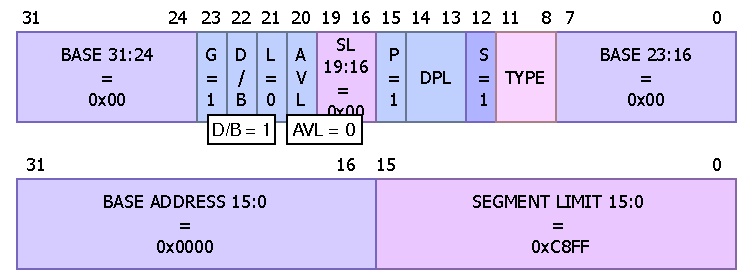
\includegraphics[scale=0.8]{img/GDTdescriptor.pdf}
	\caption{Esquema general de un descriptor de la GDT para los 4 segmentos.}
\end{figure}


\justify
Realizando lo pedido en el item b, pasamos a modo protegido. Para poder hacer esto modificamos el archivo \textbf{kernel.asm}, allí deshablitamos las interrupciones, habilitamos A20, cargamos en el registro GDTR la estructura \textbf{gdt_descriptor_t} y modificamos el ultimo bit del registro de control CR0, es decir, seteamos en 1 el bit de \textit{Protection Enable}. Posteriormente, escribimos el código necesario para saltar efectivamente a modo protegido. Debido a que este salto se consigue haciendo un \textit{far jump} a la próxima instrucción, designamos una etiqueta llamada \textbf{modo_protegido} a partir de la cual obtendremos el offset, mientras que como selector utilizamos el correspondiente al segmento de código de nivel 0. Además, seteamos la pila del Kernel en la dirección 0x25000, es decir, en la base de la pila. Una vez que pasamos a modo protegido, cargamos correctamente los selectores de segmento, en los registros ds, es, fs, gs, ss, usando como registro auxiliar ax, donde se encontraba el selector de segmento de datos de nivel 0 (RPL = 0).


\justify
Seguidamente, definimos otra entrada en la GDT destinada a un segmento de vídeo de nivel 0 (DPL = 0). A diferencia de los cuatro segmentos anteriores, la base de este segmento es distinta de 0, por lo que los campos de la base fueron completados con el valor 0x000B8000. Como la pantalla es de 80x50 y como cada pixel ocupa 2 bytes, el límite de este segmento es 0x01F3F. Como este límite entra en 20 bits, el bit de granularidad de este descriptor queda en 0. Además, al ser un segmento de datos de lectura y escritura el tipo es 0x02 y el bit de s queda seteado en 1. Como en las entradas anteriores, los bits de AVL y L quedan en 0, mientras que los bits de present y D/B quedan en 1.  

\begin{figure}[h]
	\centering
	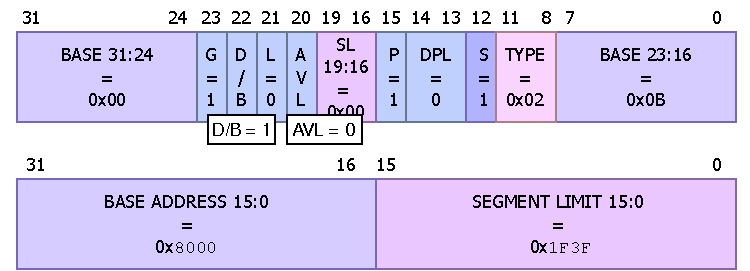
\includegraphics[scale=0.8]{img/DescriptorVideo.pdf}
	\caption{Esquema del descriptor de segmento de video.}
\end{figure}

\justify
Para finalizar este ejercicio, realizamos un rutina encargada de limpiar la pantalla, y pintar el área del mapa de color verde, junto con las barras de los jugadores Rick y Morty. Inicialmente, esta rutina fue implementada en ASM dentro del archivo \textbf{kernel.asm}, para corroborar el correcto funcionamiento del acceso al segmento de vídeo, pero luego fue reemplazada por la función en C ``inicializar_pantalla"\ que se encuentra en el archivo \textbf{screen.c}. La pantalla se ve de la siguiente manera:

\begin{figure}[h]
	\centering
	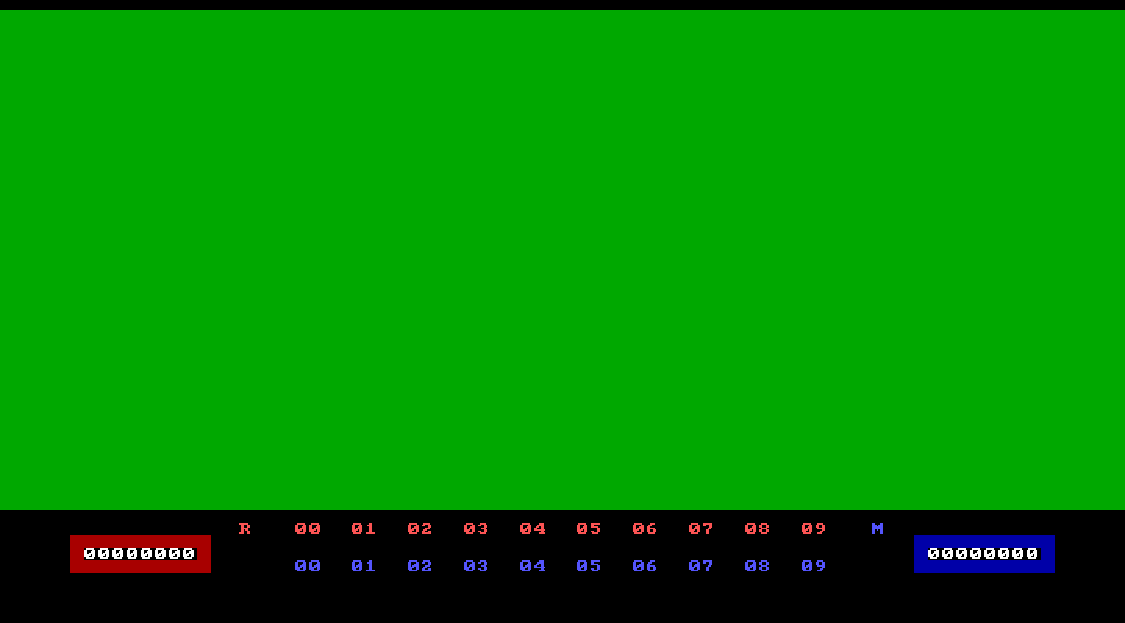
\includegraphics[scale=0.6]{img/Pantalla.pdf}
	\caption{Pantalla inicial.}
\end{figure}


\subsection{Ejercicio 2}
\justify
Inicialmente modificamos los archivos \textbf{idt.c} e \textbf{idt.h} para completar las entradas de la IDT. Definimos a la IDT como un arreglo de \textbf{idt_entry_t} de 255 posiciones, que primero inicializamos en cero, y el descriptor de la IDT (IDT_DESC), indicando el tamaño y la dirección de la IDT. Para inicializar las entradas de la IDT utilizamos un \textit{DEFINE} que, dado el número de la interrupción, completa los campos del descriptor de la IDT correspondiente. Para el caso de las interrupciones de software el DPL es 3, dado que las mismas deben poder ser accedidas por las tareas y en los demás casos el DPL es 0, ya que no deben poder ser accedidas por las tareas. En todos los casos el selector de segmento es de código de nivel 0. El bit P queda seteado en 1 y el tipo es el correspondiente a una Interrupt Gate de 32 bits (01110b). Como la dirección de las rutinas de atención (declaradas en \textbf{isr.h}) no están definidas en tiempos de compilación fue necesario definir una función llamada \textbf{idt_init} que inicializara las entradas de la IDT en tiempos de ejecución. Definimos 21 entradas en la IDT para las excepciones del procesador(de 0 a 20).
\justify
Para imprimir las excepciones en la esquina superior izquierda de la pantalla  cuando estas ocurren, implementamos la función ``print_exception", que se encuentra en el archivo \textbf{screen.c}. La misma es llamada inicialmente en el código de \textbf{isr.asm}, aunque luego esto será modificado como se ve en el código, ya que esta acción será realizada por el modo debug. 


\begin{figure}[h]
	\centering
	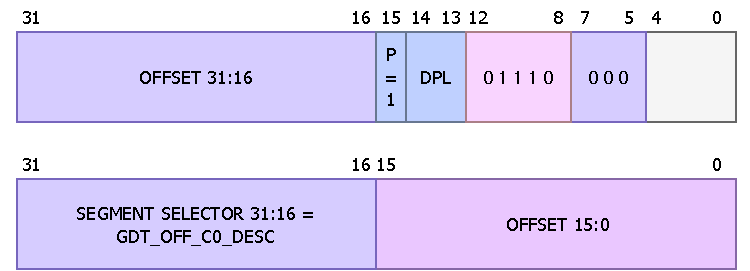
\includegraphics[scale=0.7]{img/IDTdescriptor.pdf}
	\caption{Esquema de descriptor de la IDT de tipo Interrup Gate.}
\end{figure}


\subsection{Ejercicio 3}
\justify
En este ejercicio definimos dos entradas en la IDT para las interrupciones externas o de hardware (32 del clock y 33 del keyboard) y cuatro entradas para las interrupciones de software(88, 89, 100, 123).
\justify
De acuerdo a lo pedido en el segundo, tercer y cuarto item, dentro del archivo \textbf{isr.asm} escribimos el esqueleto de las rutinas de interrupciones del reloj, de teclado y de software, que luego irán siendo modificadas a lo largo del transcurso de los ejercicios.


\subsubsection{Rutina de interrupción del reloj}
\justify
Esta rutina comienza con un call a la función pic_finish1, para avisar que la interrupción fue atendida. Seguidamente se llama a la función ``next_clock"\ , provista por la cátedra. La misma se encarga de imprimir por pantalla una animación de un cursor rotando en la esquina inferior derecha de la pantalla.


\subsubsection{Rutina de interrupción del teclado}
\justify
Esta rutina comienza levantando del puerto 0x60 la tecla que fue presionada durante la interrupción. Para que esta tecla sea impresa por pantalla se implementó la función ``print_digito"\ en el archivo \textbf{screen.c}. Para finalizar, hacemos un call a pic_finish1, para avisar que la interrupción fue atendida.

\subsubsection{Rutinas de interrupciones de software}
\justify
Las rutinas de interrupciones de software solo mueven a eax los números indicados por el item d, esto luego será modificado.

\subsection{Ejercicio 4}
\justify
Para inicializar el directorio y las tablas de páginas del Kernel, implementamos la función ``mmu_init_kernel_dir", que crea un directorio y una tabla de páginas (tabla_0) del tipo \textbf{page_directory_entry}  y \textbf{page_table_entry}, respectivamente. Estas estructuras fueron definidas en el archivo \textbf{mmu.h} y siguen el formato de las entradas al directorio y a la tabla de páginas. Una vez creados los inicializamos en 0.
\justify
La primera entrada del directorio (directorio[0]) va a mapear a la tabla de páginas creada y esta mapeará a todo el Kernel, por lo que completamos el campo de la base del directorio[0] con la dirección de la tabla de páginas. El privilegio de esta entrada es 0, el bit P queda seteado en 1, y el tipo es Read/Write. Una vez mapeado el directorio a la primera tabla de páginas, mapeamos la misma al Kernel, usando identity mapping. Nuevamente, el privilegio de cada entrada de la tabla de páginas es 0, el bit P queda seteado en 1 y el tipo es Read/Write. Al final de la rutina devolvemos la dirección del directorio de tablas de páginas. 
 
 \begin{figure}[h!]
 	\centering
 	\begin{subfigure}[b]{0.49 \textwidth}
 		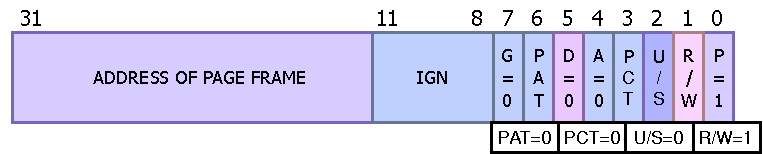
\includegraphics[width=\textwidth]{img/pde.pdf}
 		\caption{Esquema de una \textit{page directory entry}.}
 	\end{subfigure}
 	\hfill
 	\begin{subfigure}[b]{0.49 \textwidth}
 		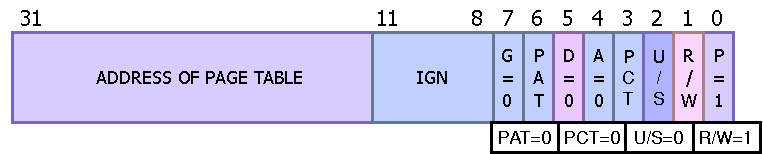
\includegraphics[width=\textwidth]{img/pte.pdf}
 		\caption{Esquema de una \textit{page table entry.}}
 	\end{subfigure}
 \end{figure}

\newpage 
\justify  
Ya creadas las funciones para inicializar el directorio y la tabla de páginas, escribimos en \textbf{kernel.asm} el código necesario para activar paginación: inicializamos el manejador de memoria y el directorio de páginas mediante un call a la función ``mmu_init" \ y ``mmu_init_kernel_dir", respectivamente. Luego, cargamos en el registro CR3 la dirección del directorio y activamos paginación seteando en 1 el bit 31 de cr0.

\begin{figure}[h]
	\centering
	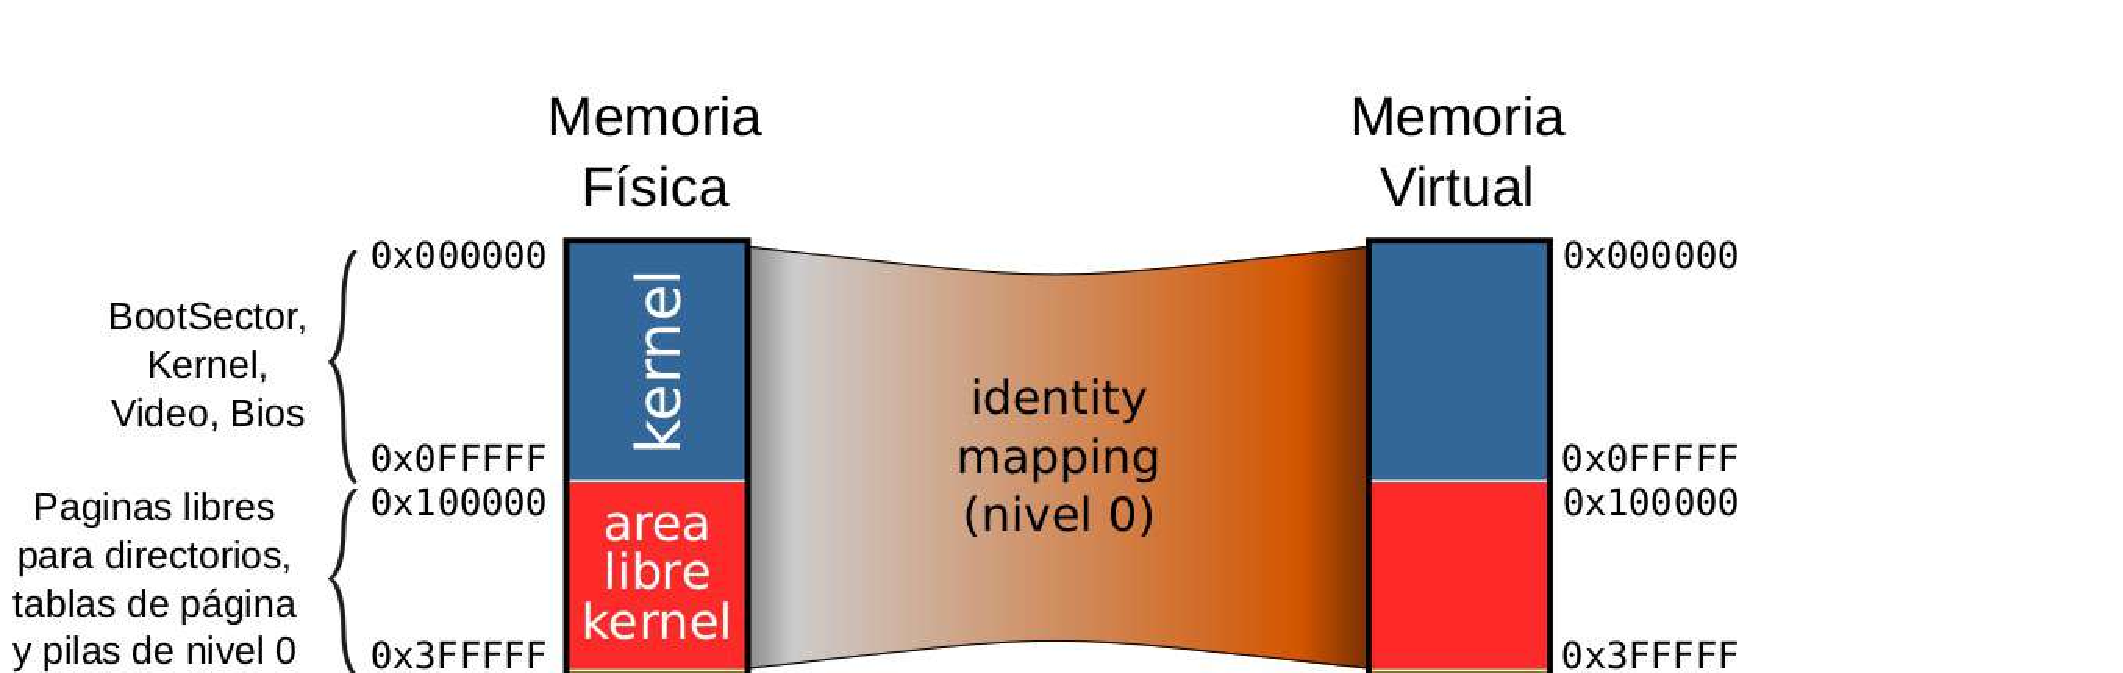
\includegraphics[scale=0.5]{img/MapearKernel.pdf}
	\caption{Mapeo del Kernel.}
\end{figure}

\subsection{Ejercicio 5}
\justify
Inicialmente y siguiendo lo indicado por el primer item, completamos la función ``mmu_init" \ con la dirección de la primera página libre del Kernel (0x100000), y luego completamos la función ``mmu_next_free_kernel_page" \ para que nos devuelva la dirección de la próxima página libre del área libre del Kernel.
\justify
Implementamos la función ``mmu_map_page" \ que, dado un CR3, una dirección virtual, una dirección fisica y unos atributos, mapea ambas direcciones. Lo primero que realiza esta función es obtener de la dirección virtual el índice del directorio de tabla de páginas y el índice dentro de la tabla de páginas. También se shiftea CR3 de tal manera de conseguir la dirección de la base del directorio. Luego, se fija si la tabla de páginas de esa \textit{page directory entry} está presente y, en caso de que no, la crea pidiendo la próxima página libre del área del Kernel y la inicializa con todas las entradas en 0. Una vez creada la tabla de páginas, se completa la entrada correspondiente de la \textit{page directory entry} con la base de la tabla de páginas y los atributos pasados por parámetro (bit de presente, bit de R/W y bit de U/S). Independientemente de si la tabla de página estaba presente o no, se obtiene la base de la página de la dirección física pasada por parámetro y se completa el campo de la base en la \textit{page table entry} correspondiente. Posteriormente, completamos la misma con los atributos pasados por parámetro. Finalmente, limpiamos la caché con la funcion tblflush, la cual fue proporcionada por la cátedra.
\justify
Implementamos la función ``mmu_unmap_page" \, la cual recibe como parámetros un CR3 y una dirección virtual, y se encarga de desmapear páginas de memoria. Al igual que la función anterior, a partir de la direccion virtual obtiene el índice del directorio de tabla de páginas y el índice de la tabla de páginas. Del CR3 obtenemos la direccion de la base del directorio de tablas y chequeamos si esa \textit{page directory entry} referencia a una tabla de páginas, es decir, posee el bit de presente en 1. En caso de no estar presente devolvemos 0. En el caso contrario, obtenemos la página que nos indica la \textit{page table entry} y le sumamos el offset de la dirección virtual. Luego, completamos esta \textit{page table entry} con 0s. Limpiamos la caché con tblflush y devolvemos la dirección física a la cual estaba mapeada la dirección virtual.
\justify
Notemos que no chequeamos si la \textit{page table entry} estaba presente, pero nosotros mantenemos el invariante de que si no está presente toda la \textit{page table entry} es 0, por ende en este caso, solo devolvería el offset de la dirección virtual.
\justify
Escribimos la rutina ``mmu_init_task_dir" \, la cual se encarga de inicializar el directorio correspondiente para una tarea Rick o Morty. Esta recibe como parámetro la dirección física donde comienza el código de la tarea (\textit{code_start}), la dirección fisica donde este debe copiarse (\textit{phy_start}) y la cantidad de páginas de código.
Para esto se crea un directorio de tablas de página pidiendo la próxima página libre de Kernel, cuya dirección será el valor del nuevo CR3. Luego, llenamos todas las entradas del directorio de páginas con 0s, y, usando la función mmu_map_page, realizamos el identity mapping del Kernel en este nuevo CR3 con los atributos P = 1, R/W = 1, y U/S = 0. Tanto en el CR3 actual como en el nuevo mapeamos 4 páginas, a partir de la dirección física \textit{phy_start}, a 4 páginas a partir de la dirección virtual 0x1D00000. Por último, tenemos que copiar el código que se encuentra en la dirección \textit{code_start} a 0x1D00000. Notemos que se realiza utilizando el CR3 actual, y por ende, luego de esto tenemos que desmapear las páginas creadas en el mismo. Finalmente, esta función devuelve el nuevo CR3.
 

\subsection{Ejercicio 6}

\justify
Nuevamente modificamos la GDT, esta vez, para agregar las entradas que serán utilizadas como los descriptores de TSS necesarios. En un principio, definimos una entrada para la tarea incial y otra entrada para la tarea Idle, cuyos índices en la GDT son 20 y 21, respectivamente. Las bases de estas fueron inicializadas en 0 para luego ser modificadas en tiempo de ejecución. El límite de ambas es 0x67 y está dado por el tamaño de la estructura de la TSS definida por la cátedra. En este caso, la granularidad está seteada en 0 por el tamaño del TSS. El bit de AVL está seteado en 0, el bit de P en 1, y el bit de DPL está seteado en 0 ya que el task switch debería poder realizarlo únicamente el Kernel. Los bits de tipo están seteados como 01001b, donde podemos ver que el bit de \textit{Busy} es 0. Los demás bits están seteados en 0 como indica el manual. Esta configuración va a ser utilizada para el resto de los descriptores de TSS.

\begin{figure}[h]
	\centering
	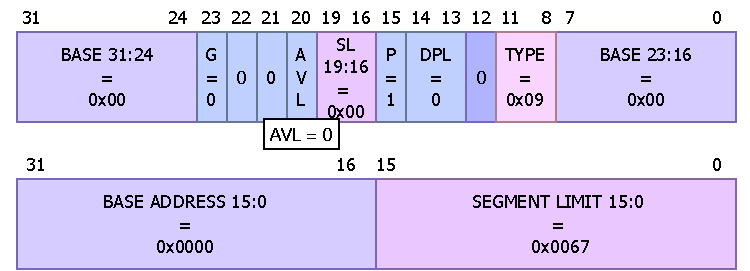
\includegraphics[scale=0.7]{img/TssdescriptorManual.pdf}
	\caption{Esquema de descriptor de la TSS.}
\end{figure}

\justify
En el archivo \textbf{tss.h} se encuentra definida una estructura que representa la TSS de una tarea que fue proveída por la cátedra. Luego, en \textbf{tss.c} definimos las TSS de la tarea inicial y la tarea Idle. La primera la llenamos con 0s y a la segunda TSS la completamos de la siguiente manera: el CR3 será igual a 0x25000 (porque comparte el mismo CR3 con el Kernel), el EIP será 0x00018000 (como indica el enunciado) y EFLAGS será 0x202 (ya que las interrupciones están habilitadas). Tanto los descriptores de datos como el de pila utilizarán el descriptor de datos de nivel 0 (RPL = 0) y el selector de código utilizará el descriptor de código de nivel 0 (RPL = 0). Por último, el esp y el ebp están seteados en la misma dirección que la pila del Kernel (0x00025000), como lo indica el enunciado. Los demás campos están seteados en 0, a excepción de iomap que esta seteado en 0xffff. Notemos que como utilizamos el CR3 del Kernel, todo se encuentra mapeado con identity mapping.
\justify
Para completar la base de los descriptores de TSS, implementamos una función en \textbf{tss.c} llamada define_base_tss, la cual toma como parámetros el indice en la GDT de la tarea y la dirección de la base de la TSS. También implementamos dos funciones, ``tss_init"\ y "tss_idle_init"\ , las cuales tienen como objetivo definir la tarea inicial y la tarea Idle utilizando la funcion anteriormente mencionada.
\justify
Para poder ejecutar la tarea Idle, primero en el Kernel escribimos el código necesario para completar las TSS de la tarea inicial y la tarea Idle. En un primer lugar, cargamos en el TR (\textit{Task Register}) el selector de TSS de la tarea inicial. Luego, para efectivamente realizar el task switch de la tarea inicial a la tarea Idle, realizamos un jump usando el selector de segmento de la TSS de Idle (RPL = 0).
\justify
Por último, en \textbf{tss.c} implementamos una función llamada ``tss_init_task" \, la cual se encarga de completar una TSS con los datos correspondientes a una tarea y completar la base de su descriptor. Esta función toma como parámetros el índice del descriptor de TSS de la tarea en la GDT, la dirección de la base de su TSS, la dirección de una página libre del Kernel (la cual sera utilizada para la pila de nivel $0$), el CR3 de la tarea, la dirección virtual donde comienza el código de la tarea y por ultimo la cantidad de páginas de código que posee.
\justify
Lo primero que realiza esta función es llamar a  ``define_base_tt" \ con los parámetros adecuados. Luego definimos la TSS de la siguiente manera: ESP0 es igual a la dirección de la página libre del Kernel más el tamaño de una página, ya que la pila crece al revés, SS0 se lo carga con un selector del segmento de datos de nivel 0 (RPL=0), CR3 se lo carga con el que fue pasado por parámetro, en EIP se carga la dirección virtual donde comienza el código, EFLAGS se carga con 0x202 (ya que las interrupciones están habilitadas). Ahora debemos cargar los selectores de segmentos de datos y el de pila, estos se cargan utilizando el selector de segmento de datos de nivel 3 (RPL=3) y CS se carga con el selector de segmento de código de nivel 3 (RPL=3). Luego,  cargamos ESP Y EBP con la dirección del código sumado a la cantidad de paginas del código multiplicado por el tamaño de una página. Por último, seteamos iomap en 0xffff. Los demás campos no son relevantes. 
\subsection{Ejercicio 7}
\justify
Notemos que la máxima cantidad de tareas que puede haber simultáneamente es $24$, las cuales son la inicial, la tarea Idle, Rick, Morty y 10 Mr. Meeseeks por cada uno. Aquellas a las que queremos repartir equitativamente el tiempo son Rick y Morty con sus respectivos Mr. Meeseeks. Teniendo esto en cuenta definimos una estructura llamada scheduler en \textbf{sched.h}, con los siguientes datos:
\begin{itemize}
	\item \textbf{Turno}: es un valor que nos indica si el turno es de Rick o de alguno de sus Mr. Meeseks, o el turno es de Morty o de alguno de sus Mr. Meeseeks. Es $0$ si es turno de una tarea de Rick y $1$ si es de una tarea de Morty.
	\item \textbf{last_task}: es un array de dos valores, el de la primera posición representa la ultima tarea de Rick ejecutada y en la segunda posición la ultima tarea de Morty ejecutada.
	\item \textbf{state}: es un array con 22 valores (la máxima cantidad de tareas simultáneas que nos interesan) que nos indica el estado de cada una de las tareas. Cada tarea puede estar en $3$ estados:
	\begin{itemize}
		\item \textbf{TASK_DEAD}: representa que la tarea está muerta, es decir, el scheduler no debe darle tiempo.
		\item \textbf{TASK_READY}: representa que la tarea está lista para ser ejecutada y por ende está viva.
		\item \textbf{TASK_EJEC}: representa que la tarea fue la última que se ejecutó o que se está ejecutando, sin tener en cuenta Idle.
	\end{itemize} 
	\item \textbf{idx_gdt}: al igual que el anterior es un array de 22 valores, que indica el índice del descriptor de TSS de cada una de las tareas en la GDT. Con esto, podemos obtener un selector de una TSS shifteando hacia la izquierda el índice de la tarea en la GDT.
	\item \textbf{reloj}: otro array de 22 valores que indica $4$ estados posibles (uno por cada estado del reloj) de cada una de las tareas.   
\end{itemize}
El orden de las tareas en los arrays es el indicado por la figura \ref{fig:array_tarea}. Para poder incluir todos los descriptores de TSS de cada una de las tareas, se modifico el tamaño de la GDT por 50. Este valor podría ser menor.


\begin{figure}[h]
	\centering
	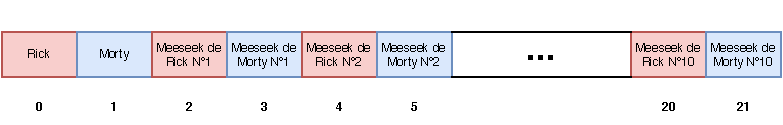
\includegraphics[scale=1.0]{img/ArrayRickyMortyIDX.pdf}
	\caption{Esquema de array de tareas}
	\label{fig:array_tarea}
\end{figure}

\justify


\justify
Ahora debemos inicializar la estructura de datos, para ello creamos un función en \textbf{sched.c} llamada ``sched_init"\ . Lo primero que realiza esta función es inicializar los estados de todas las tareas como TASK_DEAD (las tareas Rick y Morty se inician en TASK_READY en la función ``game_init" \ que luego presentaremos). Luego, inicializa los índices de cada una de las tareas en la GDT, teniendo en cuenta que los índices en la GDT respetan el mismo orden que los arrays anteriormente descritos. Por último, inicia las últimas tareas de Rick y Morty, que en este caso son las tareas principales, e inicia turno con $1$ para que el próximo turno corresponda a Rick. Los valores de los relojes están por default en 0.




\justify
Siguiendo lo indicado en el item b creamos un función ``sched_next_task"\ encargada de devolver el selector de segmento de TSS de la siguiente tarea a ejecutar. Si el juego terminó, es decir alguna tarea principal fue desalojada o si capturaron todas las Megasemillas (esto lo vamos a explicar mejor en el ejercicio $8$), devolvemos el selector de la tarea Idle. En caso contrario, el juego no terminó por ende actualizamos el estado de la última tarea que ejecutó (si sigue viva). Luego, cambiamos el turno y buscamos la próxima tarea a ejecutar que pertenezca al turno actual. Para esto, realizamos una búsqueda lineal desde la última tarea y, si nos pasamos de rango, volvemos al principio. Una vez encontrada la próxima tarea a ejecutar actualizamos last_task del turno actual. Si la siguiente tarea a ejecutar es un Mr. Meeseeks, actualizamos la máxima cantidad de casillas que se puede mover (se explicara más en el ejercicio $8$). Por último, actualizamos el estado de la próxima tarea a ejecutar, cambiamos el estado del reloj de la misma y devolvemos el selector de su TSS (RPL=0).
\justify
Para realizar el cambio de tarea, modificamos la rutina de atención del reloj (ISR 32). Definimos una variable en \textbf{isr.asm} llamada \textbf{sched_task_selector}, la cual se utiliza para guardar el selector de TSS de la tarea a la que queremos saltar y poder realizar un \textit{far jump}. Llamamos a la función ``sched_next_task"\ la cual nos devuelve en ax el resultado, es decir, la próxima tarea a ejecutar. Comparamos el resultado con el almacenado en el Task Register, para chequear si es la misma tarea. En caso de que sean iguales, no hacemos nada. Caso contrario, guardamos en \textbf{sched_task_selector} el nuevo selector de TSS y realizamos un \textit{far jump}. Como se pintan los relojes lo vamos a tratar mas adelante en el ejercicio $8$.
\justify
Análogamente, modificamos las rutinas de interrupciones de software para que salten a la tarea Idle cuando son invocadas.

\justify
Para atender a la excepciones creamos una función llamada ``sched_desalojar"\ en \textbf{sched.c}. La misma realiza una búsqueda lineal para obtener la tarea que se está ejecutando (se puede utilizar last_task y turno para realizar esto). Se actualiza el estado de la misma y en caso de que sea una tarea Mr. Meeseeks, desmapea sus páginas virtuales. Por último, llamamos a una función llamada saltar_idle() definida en isr.asm, la cual realiza un jmp far a la tarea Idle.


\justify
Para implementar el debugger utilizamos la variable debug_state. Esta puede tomar $3$ valores que nos indicaran si modo debugger esta apagado (0), activado (1) o si se esta printeando en pantalla el debugger (2).

\justify
Creamos dos funciones ``copiar_pantalla"\ y ``devolver_pantalla"\ en \textbf{screen.c} y una matriz de píxeles de 50x80 llamada copia_de_pantalla. Al llamar a ``copiar_pantalla"\ se copian los píxeles actuales de la pantalla en copia_de_pantalla y al llamar a ``devolver_pantalla"\ se pinta la pantalla con los píxeles indicados por copia_de_pantalla.
\justify
Se modificó la rutina de atención de las excepciones para que pushee todos los registros de propósito generales con un pushad, luego se pushearon los registros de segmento de datos y por último el número de excepción que ocurrió. Luego de esto, se llama a copiar pantalla, se chequea si el estado de debug_state es $1$ y en caso de que lo sea se llama a ``imprimir_debug"\ que se encuentra definido en \textbf{screen.c} y se actualiza el valor de debug\_state. Por ultimo, independientemente del valor de debug_state se desaloja la tarea actual llamando a ``sched_desalojar"\, la cual se encargara de saltar a la tarea Idle. Notemos que no restauramos la pila, ya que la tarea actual nunca mas será atendida por el scheduler, a menos que se la vuelva a crear si es una tarea Mr Meeseeks, pero en este caso será una tarea limpia.

\justify
La función ``imprimir_debug"\ toma como parámetros los registros de propósito general y los registros de segmento de datos al momento de atender la excepción. Notemos que todos estos registros poseen el mismo valor que tenían antes de producirse la excepción, menos el registro ESP, que es de nivel 0. Como se produjo un cambio en el nivel de privilegio, el estado de la pila antes de pushear cualquier registro en la rutina de atención de excepciones es el siguiente:

\begin{figure}[h]
	\centering
	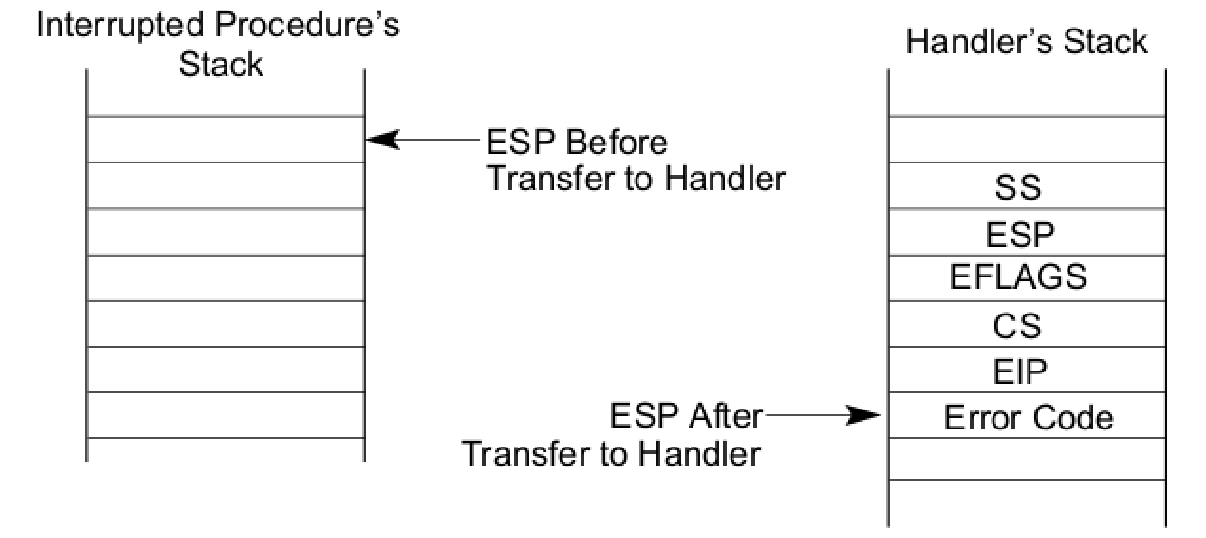
\includegraphics[scale=0.6]{img/pilaCambioPrivilegioManual.pdf}
	\caption{Stack de nivel 0 luego de un cambio de privilegio}
	\label{fig:cambio_privilegio}
\end{figure}

\justify
Ahora, queremos obtener los valores que se ven en la imagen \ref{fig:cambio_privilegio}. Cuando hacemos un pushad en la rutina de atención de una excepción, el valor de ESP que se pushea es el de antes de realizar esta operación. Por ende, los elementos que se ven en la imagen están en las posiciones siguientes al ESP pusheado. Por lo cual, podemos obtener estos valores leyendo [ESP], [ESP+4], $\dots$, pero notemos que tenemos que diferenciar si la excepción tiene código de error o no. Teniendo esto en cuenta podemos obtener los valores de la pila de nivel 0. Ahora, nos falta saber los valores de los control registers, que obtendremos a partir de las funciones provistas por la cátedra ``rcr0"\, ``rcr2"\, ``rCR3"\ y ``rcr4"\ .


\justify
Por último debemos imprimir los valores del stack y del backtrace. Para los valores del stack utilizamos el ESP de la pila de nivel $3$ de la tarea e imprimimos los $3$ primeros valores, teniendo en cuenta de estar en el rango de la tarea. Para el backtrace, usamos el ebp, asumiendo que se respeta la convención C. Con el mismo, podemos obtener con [ebp+4] la dirección de retorno de la función y con [ebp] el antiguo valor de ebp. Realizamos este proceso iterativamente 3 veces, colocando 0's si ebp o ebp+4 no estan en el rango de la tarea. Para saber si esta en el rango, utilizamos los arrays min_esp_task y max_esp_task, declarados en \textbf{game.h}, que nos indican el rango de memoria de cada tarea. Esto se puede realizar ya que estamos utilizando segmentación flat.

\begin{figure}[h]
	\centering
	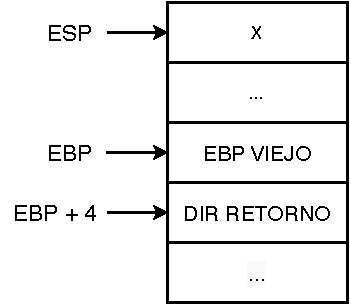
\includegraphics[scale=0.8]{img/pila.pdf}
	\caption{Pila luego del armado del stack frame}
\end{figure}


\justify
Modificamos la rutina de interrupción del teclado para que si el scan code detecta que se presiona la tecla ``Y"\ se llame a la función ``change_state_debug"\ que se encuentra definida en \textbf{sched.c}. Esta se encarga de cambiar los estados de debug_state como indica el enunciado y, si esta mostrando en pantalla el debugger, se utiliza la función ``devolver_pantalla"\ . La rutina de reloj también fue modificada para que no realice nada si debug_state es igual a $2$.


\subsection{Ejercicio 8}
\justify
Notemos que Rick y Morty pueden poseer a lo sumo 10 Mr Meeseeks simultáneamente. Las direcciones virtuales donde debe estar el código y la pila de los Mr Meeseeks es a partir de 0x08000000. Podemos entonces definir un espacio fijo para cada tarea Mr Meeseeks que se pueda crear, quedando así para cada tarea principal la siguiente asignación de espacios en su CR3:

\begin{figure}[h]
	\centering
	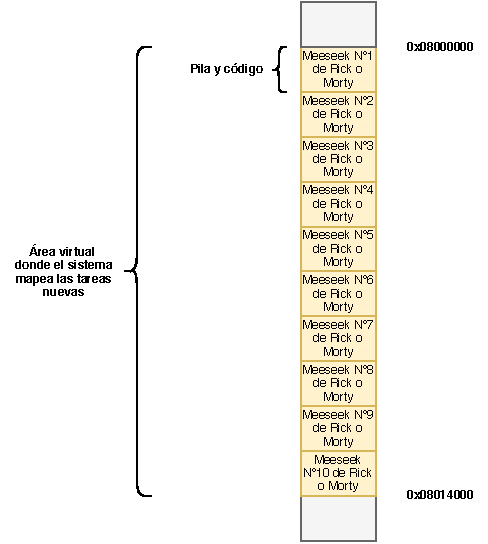
\includegraphics[scale=1.1]{img/AreaVirtualMeeseeks.pdf}
	\caption{Área virtual de los Mr. Meeseeks}
\end{figure}


\justify
Definimos las siguientes estructuras en \textbf{game.h}:
\begin{itemize}
	\item \textbf{posicion}: posee dos valores (x, y) que representan una posición en el mapa.
	\item \textbf{juego}: posee los siguientes datos:
	\begin{itemize}
		\item \textbf{posiciones_Mr_M}: un array de posiciones de tamaño 20 (igual a la cantidad máxima de tareas Mr Meeseeks), que indica en qué posición esta cada tarea Mr Meeseeks, si es que se encuentra viva.
		\item \textbf{posicion_Megasemillas}: un array de tamaño 40 (igual a la cantidad de Megasemillas iniciales), que indica en qué posición se encuentran las Megasemillas. Si la semilla no se encuentra más en el mapa se guarda el valor -1 en x e y (como son unsigend int este valor es 0xFFFFFFFF).
		\item \textbf{cant_Megasemillas}: contiene la cantidad de Megasemillas que se encuentran en el mapa actualmente.
		\item \textbf{puntajes}: es un array de dos valores. El primero indica el puntaje de Rick y el segundo el de Morty.
		\item \textbf{page_stack0_Mr_M}: es un array de tamaño 20 que contiene las direcciones de las páginas para las pilas de nivel 0 de cada tarea. Se podría usar una nueva página para cada nueva tarea que se crea, pero esto sería ineficiente ya que podemos reutilizarlas.
		\item \textbf{color_players}: es un array de dos valores. El primer valor representa el color de Rick, y el segundo el color de Morty.
		\item \textbf{max_move_Mr_M}: es un array de tamaño 20 que  indica el máximo movimiento que puede realizar cada tarea Mr Meeseeks con la syscall Move. Este valor no se guarda explícitamente, sino que cuando se crea un Mr Meeseeks en este array se guarda el valor 16. Luego, cada vez que el scheduler indique que la próxima tarea a ejecutar es un Mr Meeseeks se reduce el valor de esta tarea en el array en 1, a menos que sea igual a 2. Entonces el máximo movimiento que puede realizar un Mr Meeseeks es en realidad este valor divido $2$.
		\item \textbf{uso_portal_gun}: es un array de 20 posiciones que indica si una tarea Mr Meeseeks ya uso la syscall use_portal_gun.
		\item \textbf{cr3_players}: es un array de dos posiciones. En la primera contiene el CR3 de la tarea Rick, y en la segunda posición el CR3 de la tarea Morty.
	\end{itemize}
\end{itemize}
Los arrays que contienen datos sobre los Mr Meeseeks tendrán el siguiente orden de tareas:

\begin{figure}[h]
	\centering
	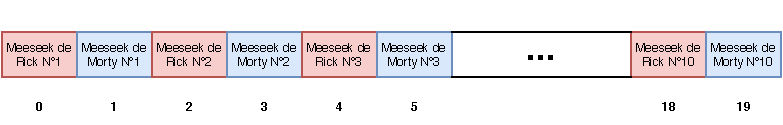
\includegraphics[scale=1.0]{img/TareasSinRickyMorty.pdf}
	\caption{Esquema de array de tareas de los Mr Meeseeks}
\end{figure}

\justify
De esta forma, dado el índice de una tarea Mr Meeseeks en el scheduler, se puede obtener el índice en estos arrays restando $2$, y también se puede obtener qué número de Mr Meeseeks es para cada tarea principal restando $2$ y dividiendo por $2$.
\justify
Implementamos la función ``game_init"\ en \textbf{game.c}, y es llamada en \textbf{kernel.asm} antes de saltar a la tarea Idle. Esta función se encarga de iniciar los arrays de puntajes y color_players; colocar las Megasemillas e iniciar cant_Megasemilla; indicar al scheduler que las tareas Rick y Morty están listas, crear su CR3 e iniciar su TSS, lo cuál se realiza con las funciones ``mmu_init_task_dir" \ y ``tss_init_task"\ ; se crean las entradas en la GDT de las tareas Meeseeks con una gdt_entry  predeterminada llamada gdt_tarea_Mr_M, la cual es similar a las entradas de las tareas Rick y Morty; se inicializa el array page_stack0_Mr_M con páginas libres del kernel. Por último, se inicializan los arrays max_esp_task y min_esp_task, los cuales indican el rango de espacio virtual de la tarea. 
\justify
Para la distribución de semillas en la pantalla del juego, en primera instancia se completa el array posicion_Megasemillas, nombrado anteriormente, con posiciones aleatorias dentro del mapa con la función ``colocar_Megasemillas"\ declarada en \textbf{game.c}. Esta función tiene en cuenta que no se creen dos semillas en el mismo lugar del mapa. Una vez hecho esto, la función ``actualizar_pantalla"\ se encarga de recorrer este array y mostrar en pantalla todas las semillas que tienen una posición válida.
\justify
Para todas las rutinas de atención de syscalls se pushean todos los registros que no tienen que devolver ningún resultado y se salta a Idle luego de llamar a la función de C encargada de realizar la operatoria. Cuando la tarea se vuelve a ejecutar, se popean los registros y se realiza un iret. Las funciones en C se encuentran definidas en \textbf{game.c}.
\justify
\subsubsection{Servicio Meeseeks}
\justify
Desarrollamos la lógica de la rutina Meeseeks con ayuda de una función en C llamada ``servicio_meeseeks". Dicha función recibe como parámetro la dirección virtual del código de un Mr. Meeseeks, y las coordenadas x e y donde el Mr. Meeseeks debe ubicarse en el mapa. En primer lugar, en esta función chequeamos que el código del Mr. Meeseeks se encuentre en el rango de direcciones de código de los jugadores; que la posición pasada por parámetro sea una posición válida en el mapa y que la tarea que llamo a la syscall no sea una tarea Mr Meeseeks. En caso de no cumplir estos requisitos, se desalojará a la tarea que llamó al servicio utilizando la función ``sched_desalojar". Posteriormente, buscamos en el array de state, el índice de una tarea muerta para asignarle a este nuevo Mr Meeseeks. En caso de no haber lugares disponibles el Mr. Meeseeks no se crea y la función devuelve 0. Luego, verificamos si en la posición donde se va a crear el Mr. Meeseeks hay una semilla con ayuda de la función ``buscar_semilla"\, la cual devuelve el índice de la Megasemilla en el array posicion\_Megasemillas, si es que existe una en esa posición, y devuelve -1 en caso contrario. En caso de que haya una Megasemilla, se aumenta el puntaje del jugador que llamó al servicio, se actualiza la información de esa semilla y se devuelve 0. Si no se cumple ninguna de las condiciones anteriores, procedemos a realizar el proceso para ubicar al Mr. Meeseeks en el mapa. Primero, actualizamos la información necesaria de esta nueva tarea en los distintos arrays mencionados anteriormente. Luego, mapeamos las dos páginas del Mr. Meeseeks creado, de acuerdo a su índice de tarea, en las dos páginas de la posición del mapa que corresponde. Una vez mapeadas, copiamos el código de la tarea, ubicado a partir de la dirección pasada por parámetro, en las direcciones virtuales recién mapeadas, teniendo en cuenta que no debemos copiar código que no se encuentra dentro del código del jugador. Luego, iniciamos la TSS de esta tarea recién creada con la función ``tss_init_task" \ , teniendo en cuenta que su código ocupa dos páginas y que la página para la pila de nivel 0 se encuentra en page_stack_0_Mr_M. Las tss de los Mr Meeseeks se encuentran en un array de tss's llamado tss\_Mr\_M de 20 posiciones, que esta declarado en \textbf{tss.c} (este posee el mismo orden que los arrays anteriores). Por último, actualizamos el estado de la tarea en el scheduler. Esta función retorna la dirección virtual de la tarea.

\subsubsection{Servicio Move}
\justify
Para desarrollar la lógica de la rutina move, nuevamente utilizamos una función en C. Esta se llama ``servicio_move"\ y toma como parámetros los desplazamientos en las coordenadas $x$ e $y$. Lo primero que realiza esta función es chequear si fue llamada por Rick o Morty, en cuyo caso se deloja a la misma con la función ``sched_desalojar". Luego, como es una tarea Mr. Meeseeks, chequeamos si el Mr. Meeseeks puede moverse dada la restricción de movimiento. En caso contrario, se devuelve 0. Si el desplazamiento en ambas coordenadas es 0, la función devuelve que el desplazamiento se pudo realizar y no realiza nada más. En cualquier otro caso, calculamos la posición final a donde debería desplazarse el Mr. Meeseeks utilizando la función de módulo(\%) de C . De manera similar a la función anterior, chequeamos si hay una semilla en la posición del mapa donde quiere desplazarse el Mr. Meeseeks. Si hay una semilla, actualizamos la información de las semillas y los puntajes, y desalojamos la tarea con la función ``sched_desalojar". En caso contrario, se utiliza la función ``move_code_Mr_M" \ para copiar el código de las dos páginas correspondientes a la celda donde se encuentra actualmente el Mr. Meeseeks hacia las dos páginas de la celda donde va a moverse. Esta función está implementada en \textbf{mmu.c} y toma como parámetro las direcciones físicas de las celdas. Lo que hace la función es mapear las páginas de ambas celdas con identity mapping en el CR3 de la tarea actual, copiar el contenido de una celda hacia la otra, y por último desmapear las páginas mapeadas. Notemos que las direcciones donde se encuentran las celdas del mapa no se utilizan para mapear ninguna otra dirección. Como la tarea Mr. Meeseeks ya fue creada, tenemos que remapear las direcciones virtuales, donde se encuentra el código de la tarea, hacia las direcciones de la celda donde se movió. Por último, se actualiza la posición del Mr. Meeseeks en el array posiciones_Mr_M, y se devuelve que se pudo mover.

\subsubsection{Servicio Look}
\justify
Para implementar la lógica de la rutina look utilizamos dos funciones en C llamadas ``servicio_look_x"\ y ``servicio_look_y", las cuales nos devuelven el desplazamiento en $x$ y en $y$ necesario para alcanzar a la semilla más cercana desde la posición del Mr. Meeseeks que llamó al servicio. Lo primero que hacemos en ambas funciones es chequear si la tarea que llamó al servicio es una tarea Rick o Morty, en cuyo caso, devolvemos -1. En caso contrario, se llama a la función ``semilla_mas_cercana" que está implementada en \textbf{game.c}, la cuál devuelve la semilla que se ubica a menor distancia Manhattan (desempata por posición en el array) realizando una búsqueda lineal en el array posicion_Megasemillas. Para finalizar, calculamos la diferencia entre las coordenadas de la semilla y el Mr. Meeseeks, y devolvemos este valor.

\subsubsection{Servicio Portal gun}
\justify
Para la rutina de use_portal_gun utilizamos la función ``servicio_portal_gun", la cuál no toma ningún parámetro. Al principio de esta función, chequeamos todos los casos en el que la misma no realiza ninguna acción. Estos son: el caso de que la tarea actual sea Rick o Morty; el caso de que el servicio de portal gun ya haya sido utilizado por esta tarea, si esto no ocurre, se actualiza el array uso_portal_gun; y el caso de que el jugador contrario no posea tareas Mr. Meeseeks vivas. Elegimos un Mr. Meeseeks random del jugador contrario mediante la función ``random_task_rival"\, la cual devuelve una tarea Mr. Meeseeks random del jugador rival, y en caso de que no exista ninguna viva retorna la tarea del jugador rival. Creamos una posición random en el mapa, si esta coincide con la posición del Mr. Meeseeks del rival, la función termina. Luego, nos fijamos si existe una megasemilla en la posición donde se moverá al Mr. Meeseeks del rival, y en el caso de que esto ocurra, actualizamos la información de las Megasemillas y el puntaje del otro jugador. También, se actualiza el estado de la tarea en el scheduler y se desmapean sus páginas virtuales en el CR3 del otro jugador. En caso de que no haya una semilla, se utiliza la función ``move_code_Mr_M"\  para copiar el código de la tarea Mr. Meeseeks del rival, desde la celda en la que se encuentra hacia la celda objetivo. Para finalizar, se remapean sus páginas virtuales hacia la nueva celda y se actualiza su posición en el array de posiciones_Mr_M.
\justify
Para dibujar los elementos de la pantalla se utilizó la función ``actualizar_pantalla"\ implementada en \textbf{screen.c}, la cuál se llama en la rutina de atención del reloj, cada vez que el debugger no está imprimiendo nada por pantalla. Dicha función realiza las siguientes acciones: actualiza las posiciones de las semillas y los Mr. Meeseeks, printea el ganador si es que el juego terminó, actualiza los puntajes y printea los relojes. En caso de que una tarea este muerta, en vez de un reloj se imprime una X.
\end{document}

